\documentclass{article}

\usepackage{amsmath,graphicx,fullpage,parskip}
\newcommand{\unit}[1]{\ensuremath{\, \mathrm{#1}}}

\pagestyle{plain}
\numberwithin{equation}{section}

\begin{document}

\title{ECE1336 Semiconductor Physics: Assignment 3}
\author{Samuel Huberman (ID 999157923)}
\date{2011-09-30}
\maketitle

\section*{Problem 1}

The potential energy from the Coulomb interaction can be represented as follows:
\begin{align*}
	E_p&=\Sigma \frac{q_iq_j}{4\pi\epsilon_0 r_{ij}}
\\	   &=\frac{e^2}{4\pi\epsilon_0}(\frac{-1}{\parallel \vec{r} \parallel}+\frac{1}{\parallel\vec{R} \parallel}+\frac{-1}{\parallel \vec{r-R} \parallel})
\end{align*}
Plotting $E_p(r)$:


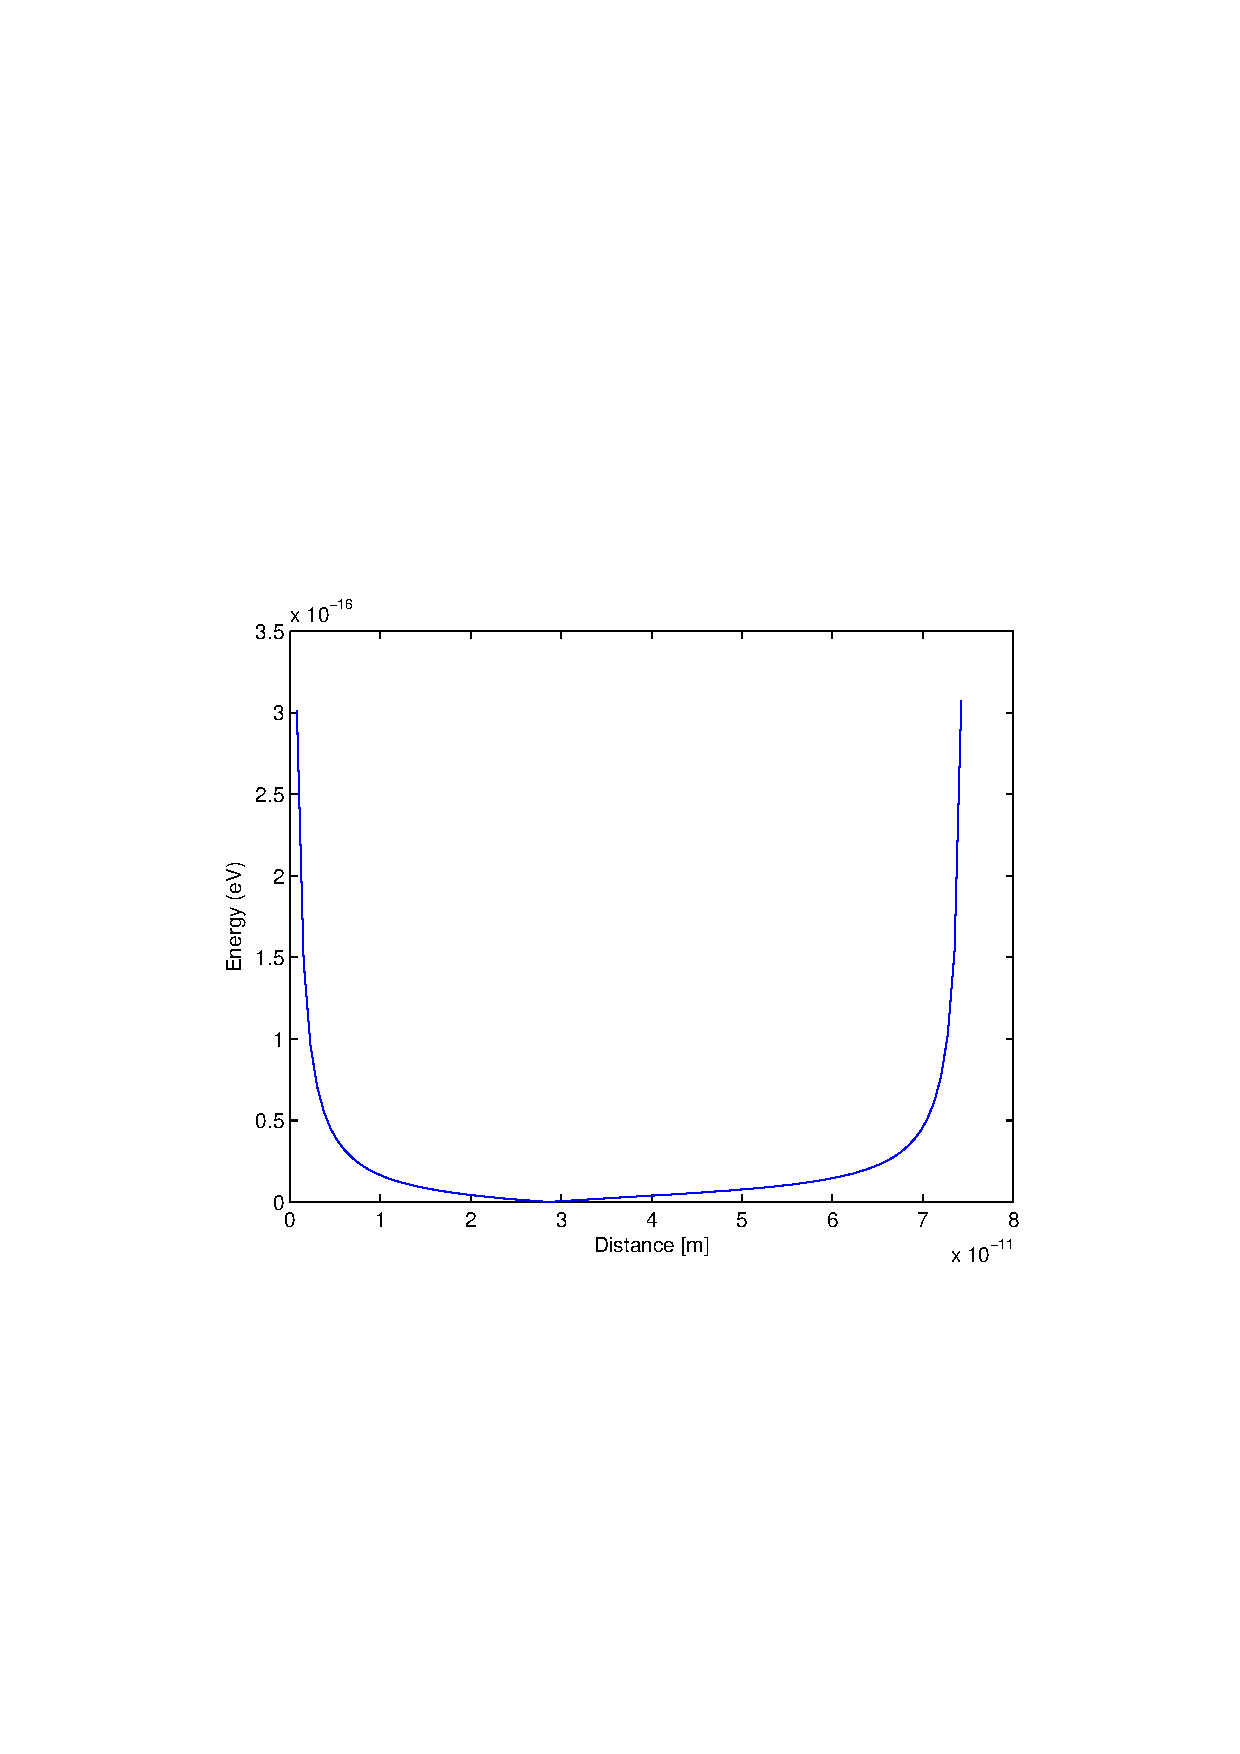
\includegraphics[scale=0.5]{A3q1.jpg}


\section*{Problem 2}
Equilibrium is achieved when the total energy of the two argon atoms is at a minimum:
\begin{align*}
	E&=-C(\frac{a_0}{R})^6+B(\frac{a_0}{R})^{12}\\
	\frac{dE}{dR}&=6C\frac{a_0^6}{R^7}-12B\frac{a_0^{12}}{R^{13}}
\end{align*}
Setting the latter equation equal to zero and solving for $R_{eq}$:
%(http://www.wolframalpha.com/input/?i=%282*1.69E8*+%285.2917721092E-11%29^6%2F2.35E3%29^%281%2F6%29$)
\begin{align*}
	R_{eq}&=(\frac{2Ba_0^6}{C})^{1/6}\\
	  &=3.8303e-10[m]
\end{align*}
The cohesive energy at equilibrium is defined the difference between the energy of atomic argon (infinite seperation) and solid argon:
%($http://www.wolframalpha.com/input/?i=-2.35E3*%28%285.2917721092E-11%29%2F3.830387E-10%29^6%2B1.69E8*%28%285.2917721092E-11%29%2F3.830387E-10%29^12$)
\begin{align*}
	E&=-C(\frac{a_0}{R_{eq}})^6+B(\frac{a_0}{R_{eq}})^{12}\\
	 &=-0.008169[eV]
\end{align*}
Therefore, 0.008169 eV is required to dissociate the equilibrium argon atoms into neutral atoms. 


\section*{Problem 3}
\begin{itemize}
\item(a) Ionic bonding is relatively strong compared to Van der Waals bonding. Both are the result of polarization: ionic bonding is due to the exchange of electron from atom to other, thereby creating a positive and negative ion while Van der Waals bonding is due to the electrostatic interaction between two electric dipoles (due to the separation of charged pairs).

\item(b) Colavent bonding occurs between the carbon atoms in the same plane, Van der Waals bonding occurs between atoms of different planes.

\item(c) Colavent bonding is a relatively strong type of bonding (compared to Van der Waals bonding), therefore a large amount of energy is required to break these bonds before the material melts. However, because of the crystal structure of Graphite where covalent bonds exist between atoms in the same plane while the weak Van der Waals exists between planes, layers of graphite can easily be peeled away.

\end{itemize}
\end{document}
